
\chapter[Evaluation of VAT using CWE-based Comparison]{Evaluation of Vulnerability Analysis Tools using CWE-based Comparison}
\label{ch:lab6} % This how you label a chapter and the key (e.g., ch:into) will be used to refer this chapter ``Introduction'' later in the report. 
% the key ``ch:into'' can be used with command \ref{ch:intor} to refere this Chapter.

\begin{center}
    \href{https://github.com/jsmaskeen/CS202-STTCSE/tree/lab6}{Github Repository for Lab 6}
\end{center}

\section{Introduction}
In this lab we evaluate and compare different static application security
testing (SAST) tools based on their ability to detect software weaknesses in
real-world, large-scale open-source projects. This comparison is based on the Common Weakness Enumeration (CWE), a community-developed list of the Top 25 most dangerous software and hardware weaknesses. By analyzing the CWEs reported by
each tool, we can see their respective strengths and weaknesses, as well as
their overall coverage of the top 25 CWEs. Furthermore, we will
use metrics such as Intersection over Union (IoU) to quantify the pairwise
agreement and disagreement between the tools, helping us understand their
similarity and diversity in vulnerability detection.

\section{Setup and Tools}
We have Git, Python, and VSCode installed. \texttt{git {-}{-}version} gives
\texttt{git version 2.45.2.windows.1} as the output. The operating system on which all commands and analysis are performed is Windows 11. SEART Search Engine
\url{https://seart-ghs.si.usi.ch/} is used to search and filter the repository
based on our criteria.
\begin{figure}[!ht]
    \centering
    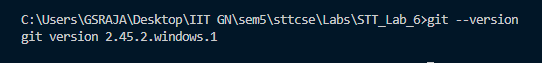
\includegraphics[width=0.5\linewidth]{figures/1_1.png}
    \caption{Git Version}
    \label{1_1}
\end{figure}
The working directory is named \texttt{STT\_Lab\_6}.

\section{Methodology and Execution}
We used the tool SEART Search Engine to search for repositories. The selection
criteria for these repositories is as follows Fig.~\ref{1_2}:
\begin{itemize}
    \item Language should be Java.
    \item There should be a minimum of 2 branches and 10 releases. (So that we can see
          the evolution of the code).
    \item The repository should have at least 10000 stars, indicating its popularity and
          activeness, and atmost 30000 stars, to avoid extremely large repositories.
    \item The repositories should have a Wiki, License, Open Issues, and Pull Requests.
\end{itemize}

\begin{figure}[!ht]
    \centering
    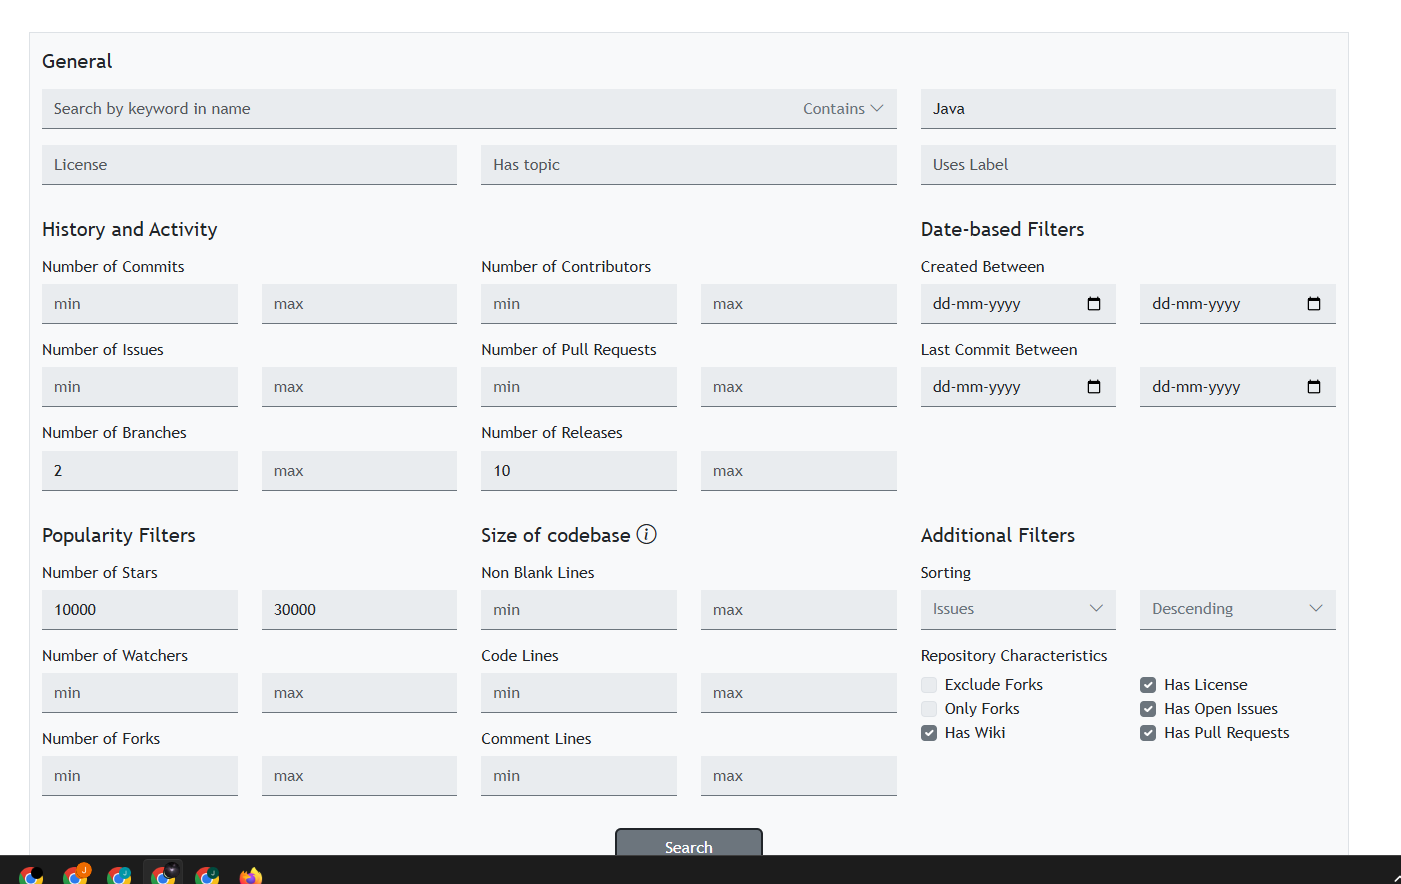
\includegraphics[width=0.8\linewidth]{figures/1_2.png}
    \caption{Search Criteria}
    \label{1_2}
\end{figure}

Based on the results, we selected three large-scale, popular open-source
repositories: \href{https://github.com/google/dagger}{\textbf{dagger}},
\href{https://github.com/google/guice}{\textbf{guice}}, and
\href{https://github.com/alibaba/sentinel}{\textbf{sentinel}}.

The following three static analysis tools, which explicitly support CWE-based
vulnerability reporting, were chosen for the evaluation:

\begin{itemize}
    \item \href{https://codeql.github.com/}{CodeQL}: A powerful semantic code analysis engine.
    \item \href{https://semgrep.dev/}{Semgrep}: A fast, open-source static analysis tool for finding bugs and enforcing code standards.
    \item \href{https://snyk.io/}{Snyk}: A developer security platform that helps to find and fix vulnerabilities in code, open source dependencies, containers, and infrastructure as code.
\end{itemize}

Each of the three selected tools were run on all three chosen projects. The
results of each scan were exported in the SARIF (Static Analysis Results
Interchange Format), which is a structured JSON format. These SARIF files are
available in the GitHub repository for this lab.

\begin{figure}[!ht]
    \centering
    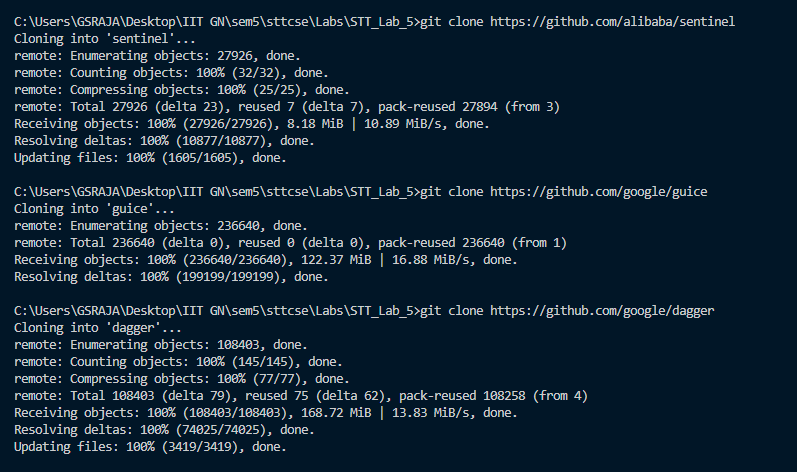
\includegraphics[width=0.6\linewidth]{figures/1_4.png}
    \caption{Cloning the chosen repositories.}
    \label{1_4}
\end{figure}

The setup for semgrep involved installing It via pip and setting an API token
(from the website) as an environment variable followed by logging in via the
command line (Fig.~\ref{1_3}). For snyk, we installed it via npm, and then set up
authentication using CLI (Fig.~\ref{1_5}). CodeQL was set up by downloading the
CLI from the official website and configuring it in the PATH.
\begin{figure}[!ht]
    \centering
    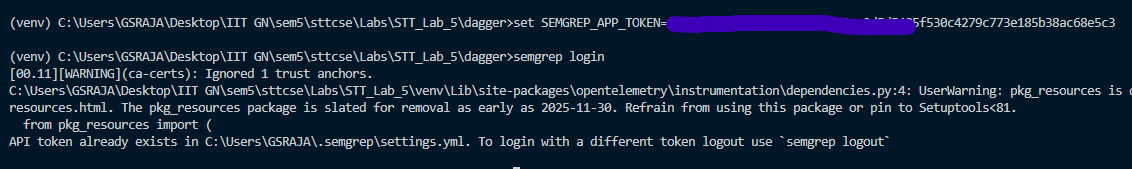
\includegraphics[width=0.98\linewidth]{figures/1_3.png}
    \caption{Semgrep Setup}
    \label{1_3}
\end{figure}

\begin{figure}[!ht]
    \centering
    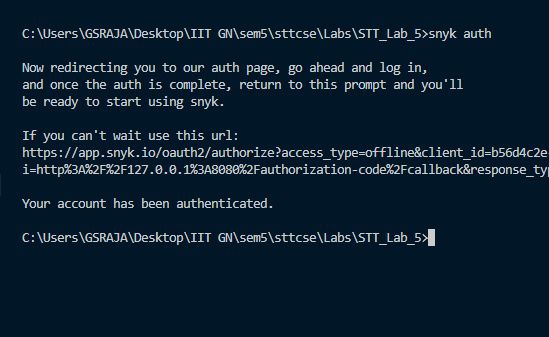
\includegraphics[width=0.6\linewidth]{figures/1_5.png}
    \caption{Snyk Setup}
    \label{1_5}
\end{figure}

We then had to build some of the repositories, for example, dagger and guice,
using \texttt{./gradle build} command (Fig.~\ref{1_8}).

\begin{figure}[!ht]
    \centering
    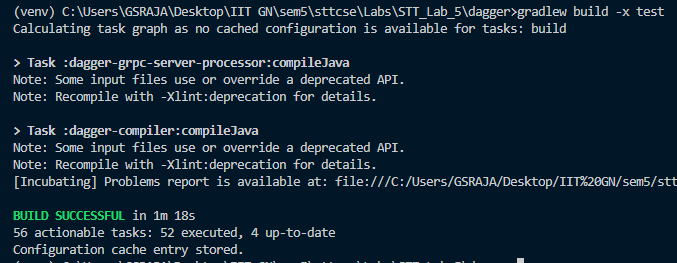
\includegraphics[width=0.8\linewidth]{figures/1_8.png}
    \caption{Gardle Build for dagger}
    \label{1_8}
\end{figure}

After building, we ran the tools on the repositories. For all three
repositories (example here, dagger), the commands used were as follows:

\begin{itemize}
    \item \textbf{CodeQL}: 
    \texttt{codeql database create ../dagger-db --language=java-kotlin}\\\texttt{--build-mode=autobuild} \\
    followed by\\
    \texttt{codeql database analyze ../dagger-db codeql/java-queries:codeql-suites/}\\\texttt{java-security-and-quality.qls --format=sarif-latest --output=codeql\_dagger-results.sarif}
    
    \item \textbf{Semgrep} (Fig.~\ref{1_7}): 
    \texttt{semgrep --config=auto ../dagger --json }\\\texttt{--output=semgrep\_results\_dagger.sarif}
    
    \item \textbf{Snyk} (Fig.~\ref{1_6}): 
    \texttt{snyk code test --sarif-file-output=../snyk\_results\_dagger.sarif}
\end{itemize}

\begin{figure}[!ht]
    \centering
    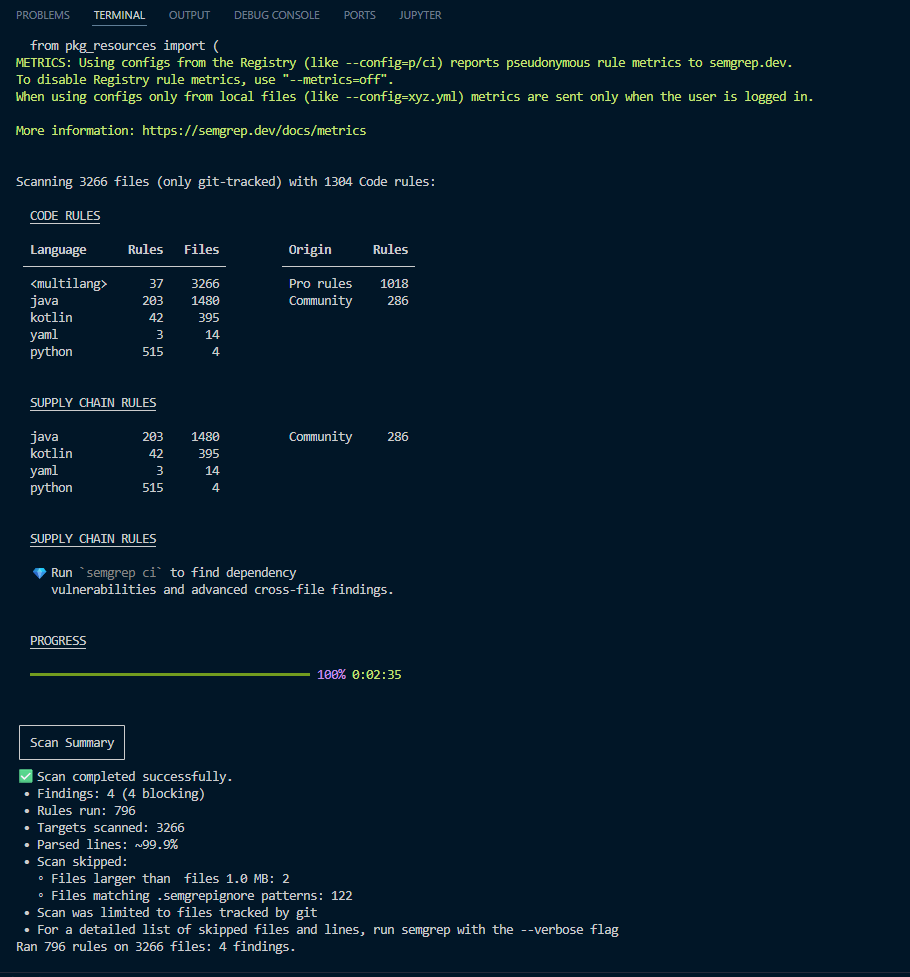
\includegraphics[width=0.8\linewidth]{figures/1_7.png}
    \caption{Semgrep Run for dagger}
    \label{1_7}
\end{figure}

\begin{figure}[!ht]
    \centering
    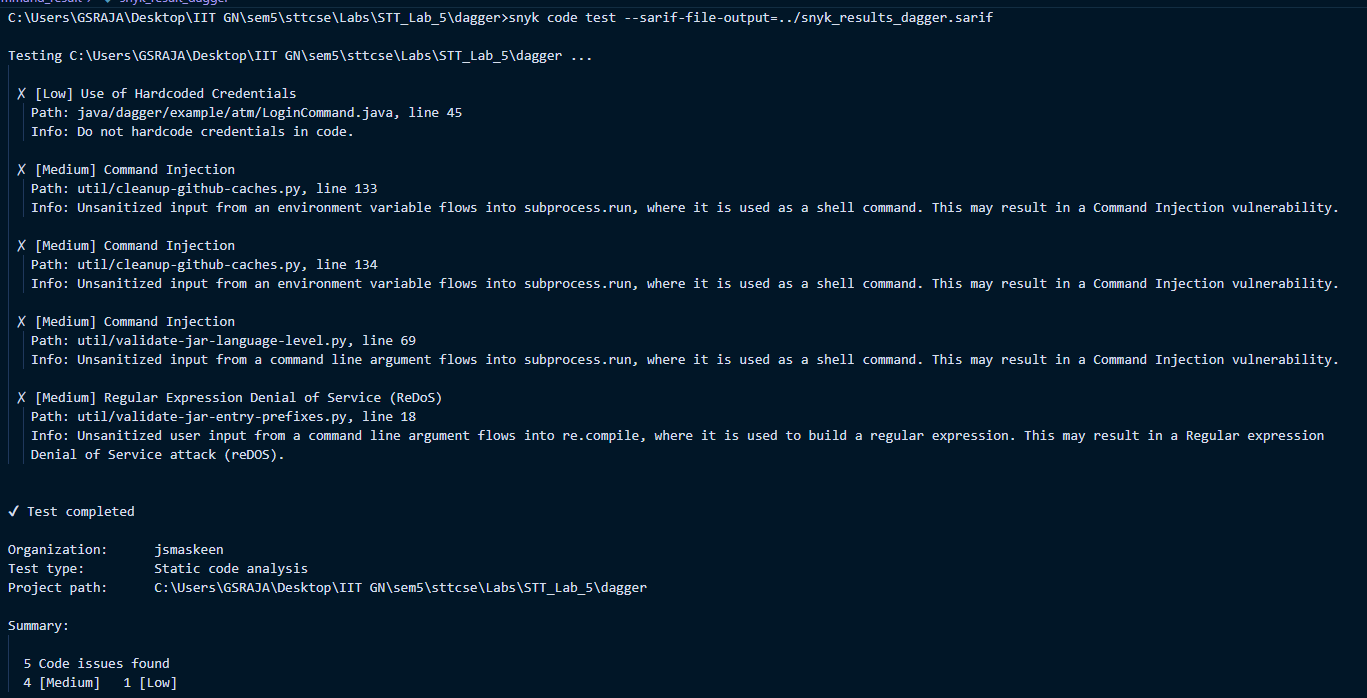
\includegraphics[width=0.97\linewidth]{figures/1_6.png}
    \caption{Snyk Run for dagger}
    \label{1_6}
\end{figure}

Note that CodeQL run for dagger had a very long output, so the STDOUT was
stored as a file, available on the github repository.

We also write a ipynb notebook to parse the SARIF files and extract the CWE IDs
reported by each tool for each repository. The findings were aggregated for
each project-tool combination, counting the number of occurrences for each
detected CWE ID. This data was consolidated into a single CSV file with the
columns: \textbf{Project\_name}, \textbf{Tool\_name}, \textbf{CWE\_ID}, and
\textbf{Num\_findings}. Additionally, each CWE ID was checked against the 2024
CWE Top 25 list, and a boolean column \textbf{Is\_in\_top\_25\_CWE} was added to
the csv to indicate whether the finding belongs to this critical set of
vulnerabilities.

We also store a csv file to show the overall coverage of each tool across all
three projects, indicating the total number of unique CWE IDs detected by each
tool againt all top 25 CWEs.

Finally, we calculated the Intersection over Union (IoU) metric for each pair
of tools across all three projects. The IoU was computed as the size of the
intersection of the sets of CWE IDs detected by each tool divided by the size
of the union of these sets. This metric tells us about the agreement and
disagreement between the tools in terms of the vulnerabilities they detect. We
plot these as venn diagrams for visual clarity.

\section{Results and Analysis}

We obtain the top 25 CWEs from
\url{https://cwe.mitre.org/data/csv/1430.csv.zip}.

\subsection{Pairwise findings}

A sample of pairwise findings for the three tools across all three projects is
shown in the table below (Table~\ref{table:findings}). The complete findings
are available in the GitHub repository.

\begin{table}[!ht]
    \centering
    \begin{tabular}{lllll}
        \hline
        Project  & Tool    & CWE ID   & Num Findings & In Top 25 CWE \\
        \hline
        dagger   & CodeQL  & cwe-248  & 2            & False         \\
        dagger   & CodeQL  & cwe-312  & 14           & False         \\
        dagger   & Semgrep & cwe-78   & 3            & True          \\
        dagger   & Semgrep & cwe-798  & 1            & True          \\
        dagger   & Snyk    & cwe-400  & 2            & True          \\
        dagger   & Snyk    & cwe-78   & 6            & True          \\
        guice    & CodeQL  & cwe-476  & 10           & True          \\
        guice    & CodeQL  & cwe-477  & 4            & False         \\
        guice    & Semgrep & cwe-489  & 2            & False         \\
        guice    & Snyk    & cwe-1004 & 2            & False         \\
        guice    & Snyk    & cwe-23   & 2            & False         \\
        sentinel & CodeQL  & cwe-079  & 10           & True          \\
        sentinel & CodeQL  & cwe-117  & 74           & False         \\
        sentinel & Semgrep & cwe-23   & 4            & False         \\
        sentinel & Semgrep & cwe-319  & 2            & False         \\
        sentinel & Snyk    & cwe-208  & 2            & False         \\
        sentinel & Snyk    & cwe-23   & 14           & False         \\
        \hline
    \end{tabular}
    \caption{Sample findings (2 rows per project-tool pair).}
    \label{table:findings}
\end{table}

\subsection{Tool level CWE coverage}

Table~\ref{table:coverage} shows the overall coverage of each tool across all
three projects, indicating the total number of unique CWE IDs detected by each
tool against all top 25 CWEs. The CWE IDs are truncated for readability.

\begin{table}[h]
    \centering
    \begin{tabular}{lllll}
        \hline
        Tool    & CWE IDs Detected (truncated)                   & Top 25 CWEs Covered & Coverage (\%)  \\
        \hline
        CodeQL  & \{cwe-571, cwe-209, \ldots\} & 5                   & 20.0                      \\
        Semgrep & \{cwe-79, cwe-319, \ldots\}   & 3                   & 12.0                  \\
        Snyk    & \{cwe-79, cwe-1004, \ldots\} & 6                   & 24.0                 \\
        \hline
    \end{tabular}
    \caption{Coverage of Top 25 CWEs by different tools (CWE list truncated for readability).}
    \label{table:coverage}
\end{table}

As shown in the bar chart below (Fig.~\ref{1_9}), Snyk has the highest coverage
of the CWE Top 25 at 24\%, followed by CodeQL at 20\%, and Semgrep at 12\%.

To visualize the specific CWEs detected by each tool, a heatmap was generated
(Fig.~\ref{1_10}), showing the coverage of each tool against the CWE Top 25
list.

\begin{figure}[!ht]
    \centering
    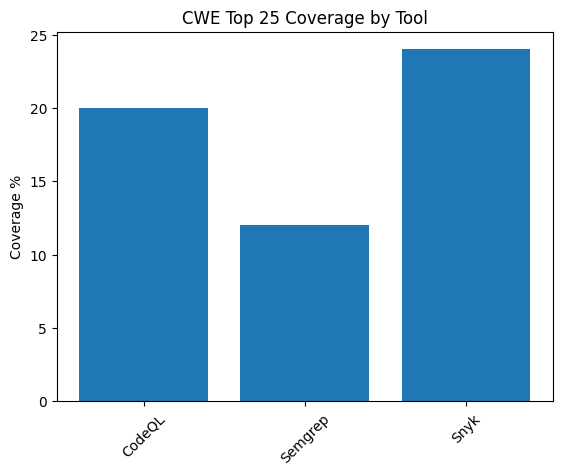
\includegraphics[width=0.5\linewidth]{figures/1_9.png}
    \caption{Bar chart showing coverage of Top 25 CWEs by different tools.}
    \label{1_9}
\end{figure}

\begin{figure}[!ht]
    \centering
    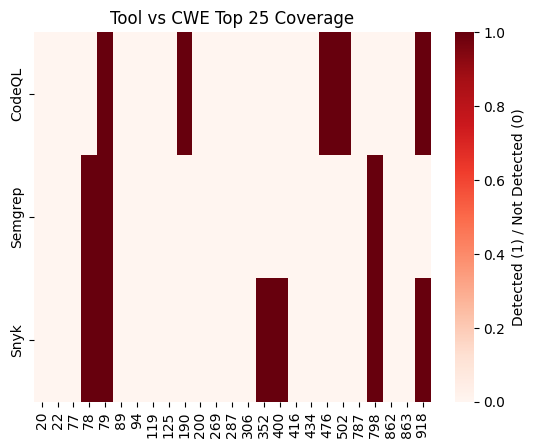
\includegraphics[width=0.4\linewidth]{figures/1_10.png}
    \caption{Heatmap showing coverage of each tool against the CWE Top 25 list.}
    \label{1_10}
\end{figure}

\subsection{Pairwise IoU Analysis}

To understand the similarity and diversity of the tools, we computed the
Intersection over Union (IoU), also known as the Jaccard Index, for each pair
of tools on a per-project basis. The IoU value ranges from 0 to 1, where 1
indicates perfect agreement (the tools find the exact same set of CWEs) and 0
indicates no agreement (the tools find completely different sets of CWEs).

\subsubsection{Dagger project}
The IoU values for the dagger project are as follows:

\begin{table}[!ht]
    \centering
    \begin{tabular}{lccc}
        \hline
                & CodeQL & Semgrep & Snyk  \\
        \hline
        CodeQL  & 1.000  & 0.000   & 0.000 \\
        Semgrep & 0.000  & 1.000   & 0.667 \\
        Snyk    & 0.000  & 0.667   & 1.000 \\
        \hline
    \end{tabular}
    \caption{IoU for dagger project.}
\end{table}

Semgrep and Snyk show a high degree of agreement (IoU = 0.667), indicating that
they detect a similar set of vulnerabilities. CodeQL, on the other hand, shows
no overlap with either Semgrep or Snyk, suggesting it identifies a completely
different set of weaknesses in this project. The venn diagram below visually
represents this overlap (Fig.~\ref{1_11}).

\begin{figure}[!ht]
    \centering
    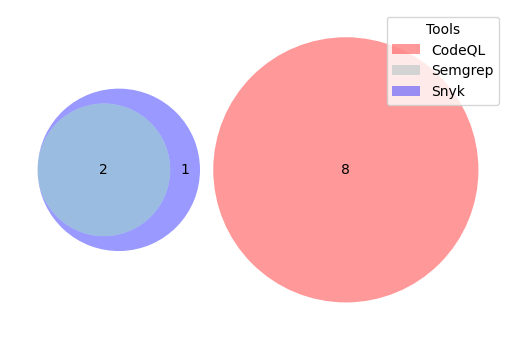
\includegraphics[width=0.5\linewidth]{figures/1_11.png}
    \caption{Venn diagram for dagger project.}
    \label{1_11}
\end{figure}

\subsubsection{Sentinel project}
The IoU values for the sentinel project are as follows:

\begin{table}[!ht]
    \centering
    \begin{tabular}{lccc}
        \hline
                & CodeQL & Semgrep & Snyk  \\
        \hline
        CodeQL  & 1.000  & 0.000   & 0.057 \\
        Semgrep & 0.000  & 1.000   & 0.200 \\
        Snyk    & 0.057  & 0.200   & 1.000 \\
        \hline
    \end{tabular}
    \caption{IoU for sentinel project.}
\end{table}

In the case of the sentinel project, all three tools show very low agreement
with each other, with the highest IoU being only 0.2 between Semgrep and Snyk.
This indicates that the tools are largely complementary for this project, each
finding a distinct set of vulnerabilities. The venn diagram below illustrates
the limited overlap (Fig.~\ref{1_12})..

\begin{figure}[!ht]
    \centering
    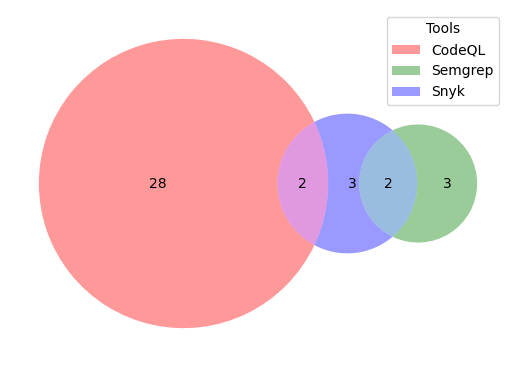
\includegraphics[width=0.5\linewidth]{figures/1_12.png}
    \caption{Venn diagram for sentinel project.}
    \label{1_12}
\end{figure}

\subsubsection{Guice project}
The IoU values for the sentinel project are as follows:

\begin{table}[!ht]
    \centering
    \begin{tabular}{lccc}
        \hline
                & CodeQL & Semgrep & Snyk \\
        \hline
        CodeQL  & 1.0    & 0.0     & 0.0  \\
        Semgrep & 0.0    & 1.0     & 0.2  \\
        Snyk    & 0.0    & 0.2     & 1.0  \\
        \hline
    \end{tabular}
    \caption{IoU for guice project.}
\end{table}

Similar to the sentinel project, the tools show low agreement for the guice
project. The IoU between Semgrep and Snyk is 0.2, and there is no overlap
between CodeQL and the other two tools. The venn diagram below visualizes this (Fig.~\ref{1_13})..

\begin{figure}[!ht]
    \centering
    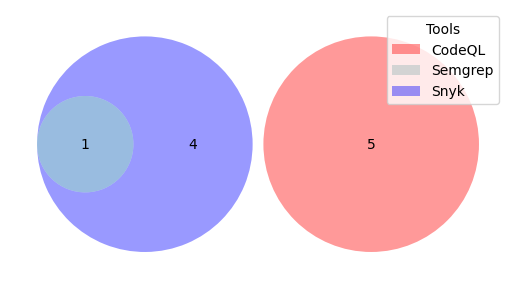
\includegraphics[width=0.5\linewidth]{figures/1_13.png}
    \caption{Venn diagram for guice project.}
    \label{1_13}
\end{figure}

\section{Discussion and Conclusion}

This lab provided us with details about the performance of different SAST
tools. Our analysis of the CWE Top 25 coverage revealed that Snyk had the
broadest coverage among the three tools. However, the IoU analysis showed that
no single tool is sufficient for in depth vulnerability detection. The low IoU
values across most tool pairs and projects highlight the diversity in their
detection capabilities.

To maximize CWE coverage, a combination of tools is necessary. Based on our
findings, using CodeQL and Snyk together would provide the best coverage for
the analyzed projects, as they tend to find different sets of vulnerabilities.
The high IoU between Semgrep and Snyk in some cases suggests that using both
might lead to redundant findings.

We understood the importance of a multi-tool approach to static analysis during
this lab. Each tool has its own strengths and focuses on different types of
weaknesses. By combining the results from multiple tools, we can achieve a more
detailed and reliable security assessment. The choice of tools should be
governed by the specific programming languages, frameworks, and types of
vulnerabilities that are most relevant to the project.

\bibliographystyle{IEEEtran}   % or any style you prefer
\nocite{*}
\bibliography{chapters/refs6}           % specific bib file for this chapter
